% ICRA two-column wrappers. Compile from this directory with pdflatex.
\documentclass[letterpaper,10pt,conference]{IEEEtran}
\IEEEoverridecommandlockouts
\usepackage{times}
\usepackage{amsmath,amssymb,bm}
\usepackage{graphicx}
\usepackage{xcolor}
\usepackage[font=footnotesize]{caption}
\usepackage{hyperref}
\hypersetup{colorlinks=false}

% Shared ICRA-style palette and TikZ keys for V19 schemes.
% Okabe--Ito accents on RLT pastel panels (colorblind-safe).
\usepackage{amsmath,amssymb,bm}
\usepackage{graphicx}
\usepackage{xcolor}
\usetikzlibrary{
  arrows.meta,
  positioning,
  fit,
  calc,
  backgrounds,
  patterns,
  shapes.geometric,
  shapes.misc,
}

\definecolor{datafill}{HTML}{F7F1E6}
\definecolor{dataedge}{HTML}{C9B89A}
\definecolor{vlafill}{HTML}{EAF3FB}
\definecolor{vlaedge}{HTML}{8FB0CC}
\definecolor{rlfill}{HTML}{EEF6F1}
\definecolor{rledge}{HTML}{7FB39A}
\definecolor{actfill}{HTML}{FFF4E0}
\definecolor{actedge}{HTML}{D4B56A}
\definecolor{obsblue}{HTML}{0072B2}
\definecolor{obsfill}{HTML}{D6E6F5}
\definecolor{rlorange}{HTML}{E69F00}
\definecolor{rltoken}{HTML}{FFCC33}
\definecolor{vlagreen}{HTML}{009E73}
\definecolor{vgfill}{HTML}{D8F0E6}
\definecolor{ink}{HTML}{1A1A1A}
\definecolor{muted}{HTML}{555555}
\definecolor{boxfill}{HTML}{FFFFFF}
\definecolor{probefill}{HTML}{F3F0FA}
\definecolor{probeedge}{HTML}{9B8FBF}
\definecolor{phaseafill}{HTML}{EEF6F1}
\definecolor{phasebfill}{HTML}{EAF3FB}

\newcommand{\zrl}{z_{\mathrm{rl}}}
\newcommand{\atil}{\tilde{a}}
\newcommand{\pihat}{\hat{\pi}}
\newcommand{\vth}{v_{\theta}}
\newcommand{\Qpsi}{Q_{\psi}}

\tikzset{
  v19/.style={
    x=1mm, y=1mm,
    >={Stealth[length=1.8mm, width=1.6mm]},
    font=\footnotesize,
    line join=round,
    line cap=round,
  },
  panel/.style={
    rounded corners=2.2mm,
    line width=0.75pt,
    inner sep=0pt,
  },
  paneltitle/.style={
    font=\small\bfseries,
    text=ink,
    anchor=north,
  },
  card/.style={
    draw=#1,
    fill=boxfill,
    rounded corners=1.2mm,
    line width=0.6pt,
    inner sep=1.5mm,
    align=center,
    font=\footnotesize,
    text=ink,
  },
  pill/.style={
    rounded corners=1.3mm,
    draw=#1,
    line width=0.55pt,
    inner sep=0.9mm,
    font=\footnotesize,
    align=center,
  },
  eq/.style={
    font=\footnotesize,
    text=ink,
    align=center,
    inner sep=0.3mm,
  },
  lab/.style={
    font=\scriptsize,
    text=muted,
    align=center,
    inner sep=0.15mm,
  },
  flow/.style={
    -{Stealth[length=1.8mm, width=1.6mm]},
    line width=0.75pt,
    draw=ink!70,
  },
  tokpipe/.style={flow, draw=rlorange, solid},
  actpipe/.style={flow, draw=vlagreen, densely dashed},
  obspipe/.style={flow, draw=obsblue, solid},
  hatchfr/.style={
    pattern=north east lines,
    pattern color=obsblue!28,
  },
}


\title{V19 schemes (not a submission)}
\author{Internal figure check}
\begin{document}
\maketitle

\begin{abstract}
Placeholder so the figure pages use IEEEtran column geometry.
\end{abstract}

\begin{figure*}[!t]
\centering
\resizebox{\textwidth}{!}{% Architecture: observation → frozen VLA + RL token → CFGRL extractor.
\begin{tikzpicture}[v19]
  \def\pw{57.4}
  \def\ph{76}
  \def\gap{4.0}

  % ========== 1. Observation ==========
  \coordinate (P1) at (0,0);
  \fill[datafill, rounded corners=2.2mm] (P1) rectangle ++(\pw,\ph);
  \draw[dataedge, panel] (P1) rectangle ++(\pw,\ph);
  \node[paneltitle] at ($(P1)+(0.5*\pw,\ph-2.0)$) {Observation};

  \node[inner sep=0.3mm, draw=dataedge, fill=white, rounded corners=0.6mm]
    (exo) at ($(P1)+(0.5*\pw,57.8)$)
    {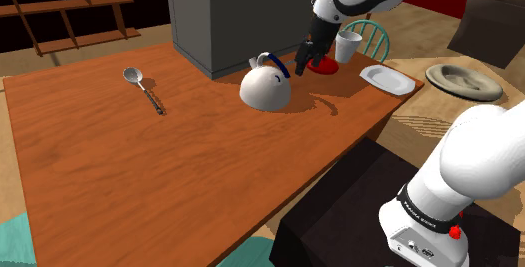
\includegraphics[width=46mm]{env/exo_kettle.png}};
  \node[card=dataedge, fill=white, inner sep=1.0mm, font=\footnotesize]
    at ($(P1)+(0.5*\pw,45.0)$) {exo RGB};

  \node[inner sep=0.3mm, draw=dataedge, fill=white, rounded corners=0.6mm]
    (wrist) at ($(P1)+(0.5*\pw,32.4)$)
    {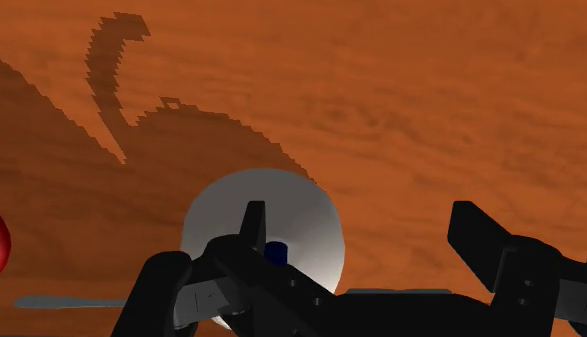
\includegraphics[width=46mm]{env/wrist_kettle.png}};
  \node[card=dataedge, fill=white, inner sep=1.0mm, font=\footnotesize]
    at ($(P1)+(0.5*\pw,20.0)$) {wrist RGB};

  \node[pill=obsblue, fill=obsfill, minimum width=21mm, minimum height=7.2mm]
    (prop) at ($(P1)+(15.0,10.0)$) {$s^{p}$};
  \node[pill=dataedge, fill=white, minimum width=29mm, minimum height=7.2mm]
    (lang) at ($(P1)+(41.6,10.0)$) {$\ell$: pick up the kettle};
  \node[lab, font=\footnotesize, text=muted] at ($(P1)+(0.5*\pw,4.0)$)
    {house0, same timestep};

  % ========== 2. Frozen VLA + RL token ==========
  \coordinate (P2) at ({\pw+\gap},0);
  \fill[vlafill, rounded corners=2.2mm] (P2) rectangle ++(\pw,\ph);
  \draw[vlaedge, panel] (P2) rectangle ++(\pw,\ph);
  \node[paneltitle] at ($(P2)+(0.5*\pw,\ph-2.0)$) {Frozen VLA $+$ RL token};

  \begin{scope}
    \clip[rounded corners=1.2mm] ($(P2)+(3.8,60.2)$) rectangle ++(49.8,9.4);
    \fill[white] ($(P2)+(3.8,60.2)$) rectangle ++(49.8,9.4);
    \fill[hatchfr] ($(P2)+(3.8,60.2)$) rectangle ++(49.8,9.4);
  \end{scope}
  \node[card=vlaedge, fill=none, minimum width=49.8mm, minimum height=9.4mm, align=center]
    (molmo) at ($(P2)+(0.5*\pw,64.9)$)
    {\textbf{MolmoAct2}  {\footnotesize(frozen)}\\[-0.15mm]
     {\footnotesize VLM $+$ flow action expert}};

  \node[font=\footnotesize, text=muted] at ($(P2)+(0.5*\pw,56.6)$)
    {last-layer tokens $\mathbf{z}_{1:M}$};
  \foreach \i/\lab in {0/$z_1$, 1/$z_2$, 2/$z_3$, 3/$\cdots$, 4/$z_M$} {
    \node[pill=obsblue, fill=obsfill, minimum width=8.0mm, minimum height=6.2mm]
      (tok\i) at ($(P2)+(10.4+8.8*\i,50.6)$) {\lab};
  }
  % token collector bar (does not share the expert pipe)
  \draw[tokpipe, -] (tok0.south) -- ++(0,-2.4) coordinate (tbarL);
  \draw[tokpipe, -] (tok4.south) -- ++(0,-2.4) coordinate (tbarR);
  \draw[tokpipe, -] (tbarL) -- (tbarR);
  \draw[tokpipe] ($(tbarL)!0.35!(tbarR)$) -- ++(0,-3.2);

  \begin{scope}
    \clip[rounded corners=1.1mm] ($(P2)+(5.6,32.6)$) rectangle ++(22.4,7.4);
    \fill[white] ($(P2)+(5.6,32.6)$) rectangle ++(22.4,7.4);
    \fill[hatchfr] ($(P2)+(5.6,32.6)$) rectangle ++(22.4,7.4);
  \end{scope}
  \node[card=rlorange, fill=none, minimum width=22.4mm, minimum height=7.4mm]
    (enc) at ($(P2)+(16.8,36.3)$) {$g_{\phi}$ (then freeze)};
  \node[pill=rlorange, fill=rltoken, minimum width=26mm, minimum height=8.2mm]
    (zrl) at ($(P2)+(16.8,24.4)$) {$\zrl\in\mathbb{R}^{256}$};
  \draw[tokpipe] ($(tbarL)!0.35!(tbarR)+(0,-3.2)$) -- (enc.north);
  \draw[tokpipe] (enc) -- (zrl);

  \node[pill=vlagreen, fill=vgfill, minimum width=24mm, minimum height=8.2mm]
    (aref) at ($(P2)+(43.2,30.6)$) {$\atil_{1:C}\sim\pihat$};
  % expert pipe goes RIGHT of the token row, never through it
  \draw[actpipe]
    (molmo.east) -- ++(2.6,0) |- (aref.east);

  \node[eq] at ($(P2)+(0.5*\pw,14.2)$)
    {$\zrl=g_{\phi}([\mathbf{z}_{1:M},e_{\mathrm{rl}}])_{M+1}$};
  \node[font=\footnotesize, text=muted] at ($(P2)+(0.5*\pw,7.6)$)
    {solid orange: tokens \quad dashed green: $\pihat$};

  % ========== 3. CFGRL extractor ==========
  \coordinate (P3) at ({2*(\pw+\gap)},0);
  \fill[rlfill, rounded corners=2.2mm] (P3) rectangle ++(\pw,\ph);
  \draw[rledge, panel] (P3) rectangle ++(\pw,\ph);
  \node[paneltitle] at ($(P3)+(0.5*\pw,\ph-2.0)$) {CFGRL extractor};

  \node[card=rledge, fill=white, minimum width=49.5mm, minimum height=8.0mm]
    (state) at ($(P3)+(0.5*\pw,64.6)$)
    {RL state $x=(\zrl,\,s^{p})$};

  \node[card=rledge, fill=white, minimum width=23.4mm, minimum height=16.0mm, align=center]
    (critic) at ($(P3)+(15.3,48.8)$)
    {\textbf{critic} $\Qpsi$\\[0.3mm]
     {\footnotesize ensemble, chunk TD}};
  \node[card=actedge, fill=actfill, minimum width=23.4mm, minimum height=16.0mm, align=center]
    (actor) at ($(P3)+(41.9,48.8)$)
    {\textbf{flow} $\vth$\\[0.3mm]
     {\footnotesize $\vth(x,a_{t},t,o)$}\\[-0.05mm]
     {\footnotesize $o\in\{\varnothing,1\}$}};

  \draw[flow] (state.south) -- ++(0,-1.6) -| (critic.north);
  \draw[flow] (state.south) -- ++(0,-1.6) -| (actor.north);

  \node[card=rledge, fill=white, minimum width=44.5mm, minimum height=13.2mm, align=center]
    (adv) at ($(P3)+(0.5*\pw+3.2,31.0)$)
    {$A(x,a)=\Qpsi(x,a)-\Qpsi(x,\atil)$\\[0.5mm]
     {\footnotesize $o{=}1$ if $A\ge 0$ or success; else $\varnothing$}};
  \node[pill=vlagreen, fill=vgfill, minimum width=8.8mm, minimum height=7.2mm, left=1.4mm of adv]
    (aport) {$\atil$};

  \node[card=actedge, fill=white, minimum width=49.5mm, minimum height=14.4mm, align=center]
    (sample) at ($(P3)+(0.5*\pw,13.4)$)
    {$v=(1-w)\,\vth(\cdot,\varnothing)+w\,\vth(\cdot,o{=}1)$\\[0.7mm]
     $\pi\propto\pihat\,p(o{=}1\mid x,a)^{w}$\\[0.4mm]
     {\footnotesize $w{=}0$ then $0.5$}};

  % Cross-panel pipes
  \draw[obspipe, line width=0.9pt] ($(P1)+(\pw,64.9)$) -- ($(P2)+(0,64.9)$);
  \draw[obspipe, line width=0.7pt]
    ($(P1)+(\pw,10.0)$) -- ++(1.5,0) |- ($(P2)+(0,64.9)$);
  \draw[tokpipe, line width=0.9pt] ($(P2)+(\pw,24.4)$) -- ($(P3)+(0,64.6)$);
  \draw[actpipe, line width=0.9pt] (aref.east) -- ($(P2)+(\pw,30.6)$) -- (aport.west);
\end{tikzpicture}
}
\caption{A frozen VLA remains the reference policy $\hat\pi$; only a compact
RL token, a chunk critic, and one CFGRL flow are trained. Guided sampling
implements the product $\pi\propto\hat\pi\,p(o{=}1\mid x,a)^{w}$ without
updating MolmoAct2.}
\label{fig:v19-arch}
\end{figure*}

\begin{figure*}[!t]
\centering
\resizebox{\textwidth}{!}{% Training loop (CPI) with brief losses. Wrap sits below the phase row.
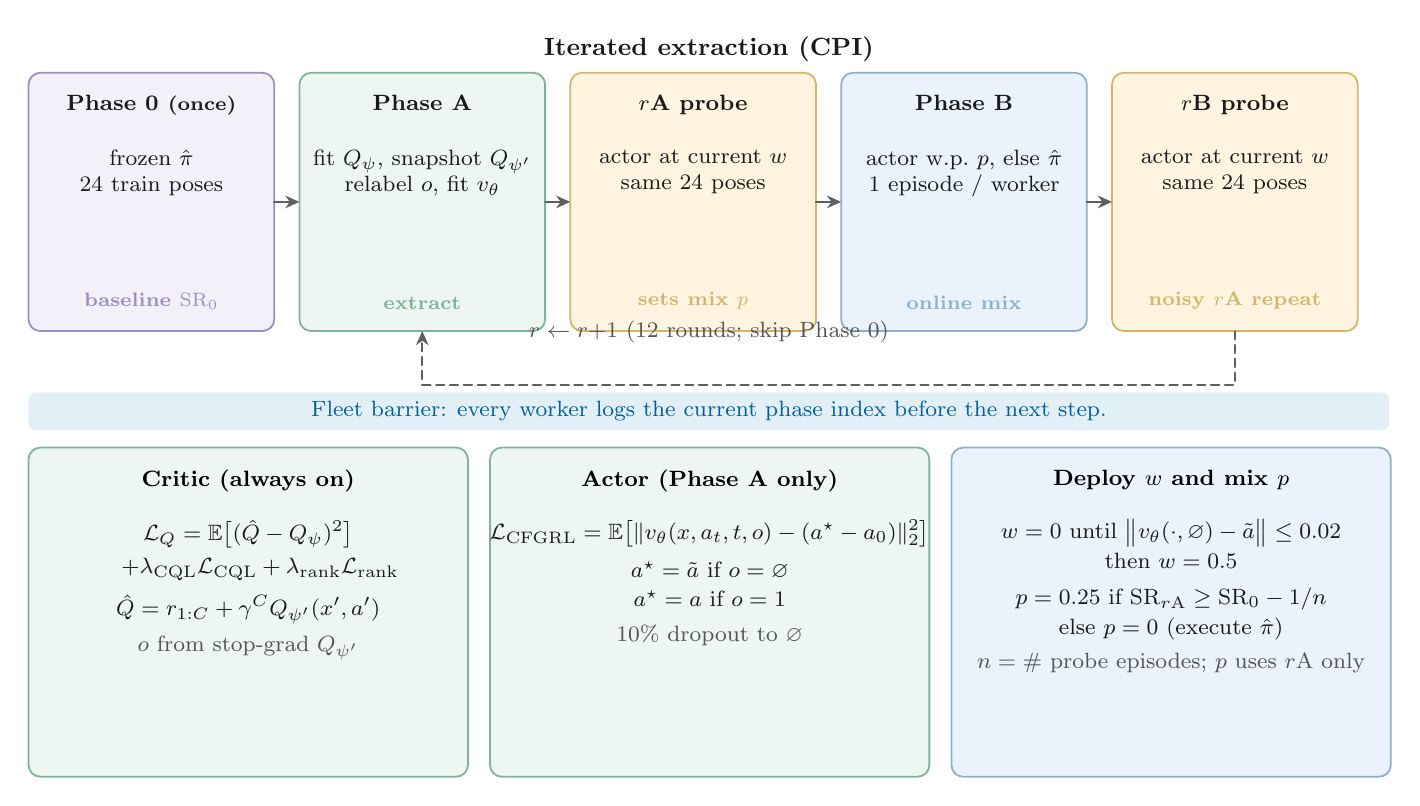
\begin{tikzpicture}[v19]
  \def\W{180}

  \node[paneltitle] at (0.5*\W,98.2) {Iterated extraction (CPI)};

  \def\bw{31.2}
  \def\bh{32.8}
  \def\by{59.6}
  \def\b0{3.6}
  \def\dg{3.2}

  \newcommand{\phasebox}[6]{% x, fill, edge, title, body, tag
    \fill[#2, rounded corners=1.5mm] (#1,\by) rectangle ++(\bw,\bh);
    \draw[#3, line width=0.65pt, rounded corners=1.5mm] (#1,\by) rectangle ++(\bw,\bh);
    \node[font=\footnotesize\bfseries, text=ink, anchor=north]
      at (#1+0.5*\bw,\by+\bh-1.6) {#4};
    \node[font=\footnotesize, text=ink, align=center, anchor=north]
      at (#1+0.5*\bw,\by+\bh-8.6) {#5};
    \node[font=\scriptsize\bfseries, text=#3, anchor=south]
      at (#1+0.5*\bw,\by+1.5) {#6};
  }

  \phasebox{\b0}{probefill}{probeedge}
    {Phase 0  {\scriptsize(once)}}
    {frozen $\pihat$\\[-0.1mm]
     24 train poses}
    {baseline $\mathrm{SR}_0$}

  \pgfmathsetmacro{\bA}{\b0+\bw+\dg}
  \phasebox{\bA}{phaseafill}{rledge}
    {Phase A}
    {fit $\Qpsi$, snapshot $Q_{\psi'}$\\[-0.1mm]
     relabel $o$, fit $\vth$}
    {extract}

  \pgfmathsetmacro{\bRA}{\bA+\bw+\dg}
  \phasebox{\bRA}{actfill}{actedge}
    {$r$A probe}
    {actor at current $w$\\[-0.1mm]
     same 24 poses}
    {sets mix $p$}

  \pgfmathsetmacro{\bB}{\bRA+\bw+\dg}
  \phasebox{\bB}{phasebfill}{vlaedge}
    {Phase B}
    {actor w.p.\ $p$, else $\pihat$\\[-0.1mm]
     1 episode / worker}
    {online mix}

  \pgfmathsetmacro{\bRB}{\bB+\bw+\dg}
  \phasebox{\bRB}{actfill}{actedge}
    {$r$B probe}
    {actor at current $w$\\[-0.1mm]
     same 24 poses}
    {noisy $r$A repeat}

  \foreach \x in {\b0,\bA,\bRA,\bB} {
    \pgfmathsetmacro{\xn}{\x+\bw}
    \draw[flow, line width=0.85pt] (\xn,\by+0.5*\bh) -- ++(\dg,0);
  }

  % Wrap under the row; label sits above the dashed line, not on it
  \draw[flow, densely dashed, line width=0.75pt]
    (\bRB+0.5*\bw,\by) -- ++(0,-6.8)
    -- (\bA+0.5*\bw,\by-6.8) -- (\bA+0.5*\bw,\by);
  \node[font=\footnotesize, text=muted, anchor=south] at (90,\by-2.8)
    {$r\leftarrow r{+}1$ (12 rounds; skip Phase 0)};

  \fill[obsblue!11, rounded corners=0.9mm] (3.6,47.0) rectangle (176.4,51.8);
  \node[font=\footnotesize, text=obsblue!85!black] at (90,49.4)
    {Fleet barrier: every worker logs the current phase index before the next step.};

  \def\ch{41.8}
  \def\cw{55.8}
  \def\cy{3.0}

  \fill[rlfill, rounded corners=1.5mm] (3.6,\cy) rectangle ++(\cw,\ch);
  \draw[rledge, line width=0.65pt, rounded corners=1.5mm] (3.6,\cy) rectangle ++(\cw,\ch);
  \node[font=\footnotesize\bfseries, anchor=north] at (3.6+0.5*\cw,\cy+\ch-1.6)
    {Critic (always on)};
  \node[eq, anchor=north] at (3.6+0.5*\cw,\cy+\ch-8.8) {%
    $\displaystyle\mathcal{L}_{Q}=\mathbb{E}\big[(\hat Q-\Qpsi)^{2}\big]$\\[0.8mm]
    $\displaystyle\quad+\lambda_{\mathrm{CQL}}\mathcal{L}_{\mathrm{CQL}}+\lambda_{\mathrm{rank}}\mathcal{L}_{\mathrm{rank}}$\\[1.5mm]
    $\displaystyle\hat Q=r_{1:C}+\gamma^{C}Q_{\psi'}(x',a')$\\[1.2mm]
    {\footnotesize\color{muted}$o$ from stop-grad $Q_{\psi'}$}
  };

  \fill[rlfill, rounded corners=1.5mm] (62.2,\cy) rectangle ++(\cw,\ch);
  \draw[rledge, line width=0.65pt, rounded corners=1.5mm] (62.2,\cy) rectangle ++(\cw,\ch);
  \node[font=\footnotesize\bfseries, anchor=north] at (62.2+0.5*\cw,\cy+\ch-1.6)
    {Actor (Phase A only)};
  \node[eq, anchor=north] at (62.2+0.5*\cw,\cy+\ch-8.8) {%
    $\displaystyle\mathcal{L}_{\mathrm{CFGRL}}=\mathbb{E}\big[\|\vth(x,a_{t},t,o)-(a^{\star}-a_{0})\|_{2}^{2}\big]$\\[1.4mm]
    $a^{\star}=\atil$ if $o=\varnothing$\\[0.4mm]
    $a^{\star}=a$ if $o=1$\\[1.1mm]
    {\footnotesize\color{muted}10\% dropout to $\varnothing$}
  };

  \fill[vlafill, rounded corners=1.5mm] (120.8,\cy) rectangle ++(\cw,\ch);
  \draw[vlaedge, line width=0.65pt, rounded corners=1.5mm] (120.8,\cy) rectangle ++(\cw,\ch);
  \node[font=\footnotesize\bfseries, anchor=north] at (120.8+0.5*\cw,\cy+\ch-1.6)
    {Deploy $w$ and mix $p$};
  \node[eq, anchor=north] at (120.8+0.5*\cw,\cy+\ch-8.8) {%
    $w=0$ until $\big\|\vth(\cdot,\varnothing)-\atil\big\|\le 0.02$\\[0.4mm]
    then $w=0.5$\\[1.3mm]
    $p=0.25$ if $\mathrm{SR}_{r\mathrm{A}}\ge\mathrm{SR}_{0}-1/n$\\[0.4mm]
    else $p=0$ (execute $\pihat$)\\[1.1mm]
    {\footnotesize\color{muted}$n=\#$ probe episodes; $p$ uses $r$A only}
  };
\end{tikzpicture}
}
\caption{Conservative policy iteration on a fixed 24-pose train set.
Phase~0 is the frozen-VLA baseline. Each round extracts a CFGRL actor,
probes it, then collects with mix $p$ against $\hat\pi$ only if that probe
is not worse than Phase~0. Guidance stays at $w=0$ until the uncond flow
matches $\tilde{a}$, then $w=0.5$.}
\label{fig:v19-loop}
\end{figure*}

\end{document}
